
\chapter{Community detection}
\label{chap:community detection}
%\todo{Mpve spinglass to end}
\todo{Expand theory of spectral clustering}

 \todo{do citations for paper before moving}





\section{Introduction}
\todo{Rewrite this section as from paper eg DH}
\textcolor{red}{start of dh intro}
Intelligence, also known as general cognitive function,\cite{davies2015genetic} or simply as g,\cite{spearman1961general} describes the finding that across seemingly-disparate measures of cognitive ability, a single common factor explains around 40\% of the total cognitive test score variance in a group with a range of intellectual ability.  \cite{carroll1993human}  This single factor is the source of much of the predictive validity of cognitive tests; higher measured intelligence is predictive of higher-level educational and occupational outcomes, \cite{strenze2007intelligence}  as well as better health, and longevity .\cite{deary2012annrev} 

In twin and family studies genetic factors explain between 50-80\% of individual differences in intelligence. Using GREML-SC implemented in GCTA, \cite{yang2011gcta}  common single nucleotide polymorphisms (SNPs) have been found explain 20-30\% \cite{marioni2014common}  of differences in intelligence. When variants that are poorly tagged by genotyped SNPs are included using GREML-KIN, \cite{xia2016pedigree}  or GREML-MSC and imputed genotypes, around 50\% of the differences in intelligence can be explained using molecular genetic data. \cite{hill2018genomic} 

Consistent with the findings from other polygenic traits such as height, \cite{wood2014defining}  the number of variants associated with intelligence has increased as sample sizes have become larger. \cite{sniekers2017genome},\cite{hill2019combined}  However, the problem remains of how to transform information pertaining to phenotype-associated genetic loci into coherent biological explanations on how genetic differences result in phenotypic differences in intelligence. One such method that has been applied to intelligence is gene-set analysis (GSA). 

The logic of GSA is to examine a group of genes that are united by a common theme such as biologically-relevant mechanisms, \cite{hill2014human}  broadly constructed functional regions of the genome, \cite{hill2016molecular}  or being associated with a related phenotype. \cite{hill2016examining}  These gene sets are then examined against genes drawn from outside of the gene-set being tested using competitive gene set analysis (for a detailed discussion. \cite{de2016statistical}  Failure to compare the genes of interest against those from outside the set (i.e. to use self-contained gene set analysis) will result in an inflation of the alpha level. \cite{de2016statistical} 

GSA has indicated that the tissues of the brain and central nervous system are enriched for association with intelligence, \cite{hill2016molecular},\cite{johnson2016systems}  and has also been used to link transcription rate of genes expressed in the brain to genetic variation using genome-wide association study (GWAS) data sets on intelligence. \cite{hill2019combined}  Additionally, the NMDA- receptor signalling complex, a component involved in synaptic plasticity, has been shown to be associated for intelligence using competitive testing. \cite{hill2014human}  More recently, neurogenesis, the process by which new neurons are formed, as well as processes involved in the myelination of the central nervous system, have been implicated as biological mechanisms that bridge the gap between genotype and intelligence differences in humans. \cite{hill2019combined}  

\textcolor{red}{end of DH intro}
Effective synaptic function depends upon protein-protein interactions between over 2000 synaptic proteins (the synaptic proteome). Genetic variations in neuronal synaptic receptor components have been found to be enriched for differences in intelligence. \cite{hill2014human}  The complexes formed by these interactions have been described as ‘molecular machines’, and are a complex system with emergent structures and properties. \cite{grant2012synaptopathies}

Complex systems such as the synaptic proteome can be modelled as a network of nodes (vertices) joined by edges (links). In a network model of the synaptic proteome the nodes are genes that encode a synaptic protein and an edge shows that the protein products of two genes (nodes) interact. A network can be analysed at three levels: the network’s properties as a whole, the properties of individual nodes, or the presence of structures or organisation within the network.  \cite{newman2012communities}   
Many complex networks such as the internet, academic collaboration networks, and protein interaction networks share common properties at the level of the entire network. These properties include the small world phenomena or scale-free degree structures\cite{barabasi1999emergence},\cite{watts1998collective}  and provide evidence on how these networks form, how information passes through them and how resilient they are to disruption. \cite{rosvall2008maps},\cite{albert2000error},\cite{bianconi2001competition}  Recently the ‘small world property’ has been posited as a potential mechanism for an omni-genic model of genetic influence on complex traits. \cite{watts1998collective},\cite{boyle2017expanded} 


Communities  are the most well studied large-scale structure in networks. \cite{newman2012communities}  Communities are connected sub-graphs with dense interactions between community members and sparser connections to the rest of the graph. \cite{newman2012communities},\cite{fortunato2016community},\cite{girvan2002community} . They are not present in random graphs and are of interest because of their functional implications: in human and animal social networks they have been shown to correspond to real world grouping in the data, and these assignments can be made solely on the pattern of connectivity of the vertices. \cite{adamic2005political},\cite{zachary1977information}  An example of a community would be a group of friends in a social network; in the synaptic protein network, communities may represent functional modules and can therefore be used as gene sets for competitive GSA.  \cite{pocklington2006proteomes},\cite{mclean2016improved}  

Metabolic networks have been shown to contain hierarchical organisation and structure.\cite{ravasz2002hierarchical} Community detection methods when applied to synaptic protein networks and combined with over-representation GSA show differential enrichment of disease and Gene Ontology terms in particular communities. \cite{pocklington2006proteomes},\cite{mclean2016improved}  GWA studies results have been analysed with GSA using communities derived from protein interactions but the analysis was confined to genes achieving genome wide significance in 70 different disorders and the protein network used interactions derived from evidence other than direct interaction (such as co-expression) and was not tissue specific. \cite{ghiassian2015disease} 
Different tissues will contain different proteins and as a result the network will have different nodes and edges. Vertex (node) statistics such as degree will therefore be different and  community detection algorithms may give different results.

Many methods require the number of communities to be known (or guessed) in advance. Pocklington used the hierarchical divisive edge betweenness community detection method described by Girvan and Newman to perform community detection on an interaction graph of the NRC/MASC complex (248 edges, 105 nodes). \cite{pocklington2006proteomes},\cite{girvan2002community}  This has the advantage that the number of communities does not have to be determined in advance, the optimum level to stop the division is determined using an objective function, the modularity (Q), to determine the quality of the division of a network into communities. \cite{girvan2002community}  Modularity is a measure of the difference between the number of edges found between members of a community and the expected number of edges given the degree of the network. This is calculated using a random model of edge generation, the configuration model, where the degree of nodes is fixed and the edges assigned at random. \cite{fortunato2016community} 

Community detection can be posed as maximising the modularity over all possible divisions of the graph to obtain non-overlapping groupings of the nodes. \cite{newman2013spectral}  Modularity maximisation is computationally hard and a number of heuristics have been described to provide approximations to the optimal modularity. \cite{newman2013spectral} With increasing graph size many of these can become unstable, give rise to improbable community sizes, or become prohibitively computationally expensive. \cite{pocklington2006proteomes},41  
McLean et al \cite{mclean2016improved}  described a parallelized implementation of the edge betweenness algorithm used on the MASC complex   and found it to be prohibitively slow with large networks.  A powerful method of community detection that scales well with network size makes use of the spectral properties of the matrix representations of the network edges. \cite{newman2013spectral}  The network can be recurrently partitioned using the sign of the leading eigenvector of the modularity matrix. \cite{newman2013spectral}  McLean et al \cite{mclean2016improved}\todo{this just about repeats the previous two sentences} provide an implementation of this algorithm along with the random walk and edge betweenness algorithms optimised for computers with multiple cores. Examining the performance of these algorithms on a graph of the PSD they concluded the spectral clustering method with a fine-tuning step provided the best performance, measured by running time, community size and differential functional enrichment. 

Here we analyse a comprehensive and curated synaptic proteome network composed of the post synaptic density and its essential protein interactors. We combine this with the spectral clustering algorithm implemented by McLean shown to produce valid, and replicable communities in postsynaptic density complexes. \cite{mclean2016improved}  The community structures found in this network were then examined, using competitive GSA, to find if genetic variation in the genes encoding their proteins had an enriched association with a measure of cognitive ability, and one that has been used as a proxy for it: intelligence, and educational attainment. We examined whether any network node statistics are correlated with gene scores for intelligence or educational attainment.

This approach allows us to test three hypotheses aimed at contributing to understanding how genetic variation leads to individual differences in cognitive ability. Firstly, we test whether communities found in the post synaptic proteome graph are enriched for SNPs that have an effect on two measures of cognitive ability. Secondly, we test whether highly-connected hub nodes or other nodes that are influential in the network are associated with differences in human cognitive ability. Finally, we test the hypothesis that genetic variations in the protein complexes that surround the receptors, rather than just the receptors themselves, “interfere with the emergent functions of the protein set‚” 18  and play  a significant role in complex traits and diseases influenced by changes in synaptic function. 

This combined approach for analysis of neuropsychiatric GWA using synaptic structure can readily be extended to other disorders. 


\section{Methods}
To study the effect of synaptic network structure on the genetics of cognitive ability and educational attainment we have used a discovery and replication cohort design. To understand how the structure of the PSP might affect the genetic architecture of these complex phenotypes, we first tested if there was an association between measures of the influence of individual vertices (gene) in the graph (degree), and their significance in GWA studies. 
Next, we used GSA to test whether the genes encoding proteins forming community structures in the network were significantly associated with differences in intelligence or educational attainment. 

\subsection{Cohorts and studies}
\section{Cohorts and samples}

The population data used to test the association of centrality measures with population studies of educationbal attainment and intelligence were those described in sections~\ref{sec:cohorts from paper section} and \ref{sec:samples from paper section}



\subsection{Community detection – choice of algorithm.} 
To divide the network into its substructures wWe used a C++ implementation of spectral clustering with a fine tuning step in this paper as it previously provided the best balance of performance and informative functional enrichment on synaptic proteome networks. \cite{mclean2016improved}  The community structure is derived only from the pattern of network connections. i.e. no functional data is used to derived the substrucures.
Community detection was carried out using the CDS package onas described in \cite{mclean2016improved} using ECDF, the distributed computing facility provided by the University of Edinburgh. All other analysis was performed on an Intel® Core™ i7-7700K CPU @ 4.20GHz 8 core workstation running Ubuntu 16.04 LTS 64 bit.  
The modularity, a measure of the quality of the community prediction results, for the network partitioning was calculated in igraph library for R \cite{csardi2006igraph} . For all code see supplemental materials. 

\subsection{Network statistics}
To test the hypothesis that measures of gene importance in the network are correlated with cognitive ability and/or educational attainment, we calculated a range of standard network measures: betweenness centrality, degree, clustering coefficient, closeness centrality and eigenvector centrality using igraph for Python 3.6. \cite{csardi2006igraph}  We calculated the correlation between each of these vertex scores and the -log10 transform of the gene level p values derived from MAGMA for each study using Spearman’s rank correlation using the Scipy stats package for Python 3.6. 
\subsection{Study design Topology based GSA}
To test the hypothesis that there are network communities with an enriched association of genetic variations for intelligence and cognitive ability we carried out the following procedures.
Communities of genes within the PSP are identified using spectral clustering. Gene based statistics are then calculated for the discovery and replication cohorts. We then use GSA to analyse data from the discovery cohorts’ GWA analyses of intelligence and cognitive ability, to identify potential communities of interest. PSP communities of interest are then tested in independent replication cohorts with correction for multiple hypothesis testing. The study design is shown in figure 1.

\subsection{Gene Based Statistics}
We calculated gene based statistics for each study using MAGMA (v1.06) using the NCBI 37.3 assembly to identify gene boundaries. \cite{de2015magma}   No window was used around the gene boundaries. Linkage disequilibrium was corrected for using 1000 Genomes European data provided by the CTG lab with the MAGMA software version 1.6.\cite{de2015magma}  Commands used for gene based tests are found in the shell script in supplementary material. Data for the meta-analysis of intelligence performed by Sniekers  et al. was downloaded from the CTG website (see urls). \cite{sniekers2017genome}  The summary statistics for the EA2 study of educational attainment were obtained from the authors and excludes UKBiobank Phase II Education data (used as the discovery cohort) in addition to the data from 23 and me. \cite{okbay2016genome}  The summary statistics unsorted by sex were used for analysis. Summary statistics for Phase II of UKBiobank Education cohort and intelligence cohort were obtained from the co-authors directly from the CCACE.[ref]\todo{get ccace ref}

\subsubsection{PASCAL}
\label{sec:PASCAL community detection}
In order to determine if the choice of software for deriving a gene-based statistic influenced our results, we repeated our analyses using PASCAL instead of MAGMA, to provide both a gene level statistic and a competitive test of gene set enrichment. \cite{lamparter2016fast}  Pascal operates in a similar way to the popular VEGAS package but with a much shorter run time and the results are comparable. \cite{lamparter2016fast},\cite{liu2010versatile}  We judged it to be prudent to use an additional gene scoring method that uses a different scoring method as all subsequent analyses are dependent upon the gene score. 1000 Genomes European data was again used to account for linkage disequilibrium and no window was included around gene boundaries. The instructions supplied to the program are available in the supplementary material as a shell script. 

\subsection{Gene set selection}
We used the non-overlapping communities generated by the spectral community detection algorithm as gene sets stored in .gmt file format (each row a gene set). We represented each protein in the community by the Entrez ID representing the gene encoding that protein. 

We selected gene sets with more than 15 members. Divisive algorithms are known to often produce numerous small communities. Small gene sets can result in the signal being dominated by a single gene. We used the default lower limit gene size for the Gene Set Enrichment Analysis software, GSEA, as the lower limit (15). 54  

\subsection{Gene-set analysis}

We carried out gene set analysis using the inbuilt GSA function implemented in MAGMA and using the non -parametric competitive method implemented in GSEA. \cite{de2015magma},\cite{subramanian2005gene}  MAGMA provides a competitive gene set analysis using the regression weight of the association of the genes in the group with the phenotype. \cite{de2015magma}  We followed the advice of Wilmot and Mooney and used more than one enrichment method utilising GSEA to provide a non- parametric enrichment analysis. \cite{subramanian2005gene},\cite{mooney2015gene}  GSEA calculates the enrichment of a set of genes by calculating a running Kolmogorov-Smirnov score weighted by the p value of the gene in the gene level analysis. The -log10 transform of the gene level p values obtained using MAGMA were used as input for GSEA. Gene set enrichment analysis was carried out using the command line interface for the Java implementation of GSEA (GSEA - 3.0). The script to carry out the gene set analysis is included in the supplemental materials. 

We had no prior belief which, if any, communities would be associated with either phenotype. We therefore identified a set of genes (community) to be of interest if it attained nominally significant enrichment when tested using MAGMA GSA and GSEA. These gene sets were then used in the replication cohort GWA studies with correction of p values for multiple testing using the MAGMA permutation test and calculation of FDR q values in GSEA. Finally, the analysis pipeline was re-run using a different method of gene and pathway scoring to test whether the findings might be dependent on a particular package using PASCAL and its associated pathway analysis platform. \cite{lamparter2016fast}  

\subsection{Gene ontology enrichment}
To investigate the nature and function of significant community modules we used gene ontology enrichment analysis (see section~\ref{sec: gene ontology analysis}). \cite{mi2013large}  

 We tested for over representation of Gene Ontology terms in significant communities (sets) for each of the major Gene Ontology clades using Fishers exact test with corrections for multiple comparisons using the FDR method calculated using PANTER 13.1.\cite{mi2013large}We tested whether terms were over represented in these communities compared to their frequency both in the whole genome (using default  PANTHER settings) and compared with the  other 3457 genes in the PSP. \cite{mi2013large}  The ToppGene enrichment package was used to perform enrichment analysis of significant communities for murine and human phenotypes. \cite{chen2009toppgene}  

\subsection{Evolutionary Constraint}

The Exome Aggregation Consortium (ExAC - Broad Institute) contains DNA sequence data from the exomes of 60,706 individuals and provides metrics to identify genes subject to strong selection pressure against mutation. \cite{lek2016analysis}  We used data from version 1 (see URLs for source). This provides gene level measures of intolerance to deleterious mutations. The post synaptic density is known to be under evolutionary constraint with a low dN/dS (amino acid change/synonymous mutation change) in both murine and human PSD. \cite{ryan2009origin},\cite{bayes2012comparative},\cite{bayes2011characterization}  A bi-map was made between Ensembl transcript id in the ExAC data download and Entrez-id for the GRCh37 assembly using BioMart. \cite{smedley2015biomart}  We used the probability of the loss of function intolerance (pLI) to measure genetic constraint.

\section{Results}

\subsection{Synaptic Proteome Graph}

The largest connected component of the graph of the postsynaptic proteome (PSP) consisted of 3457 nodes and 30498 edges. The mean degree (the number of edges incident to each node) was 17.6, the median 8, minimum degree 1 and maximum degree 535. The degree distribution is consistent with a power law distribution. Further details on the graph are available in supplemental table 3. 
\subsubsection{Spectral community detection}
65 post synaptic graph communities (clusters) were detected using the spectral clustering algorithm with fine-tuning step; the modularity (Q) of the partition was 0.30 indicating a robust community architecture.  The communities ranged in size from 1 to 405 genes (mean 53.2, median 27, standard deviation 73). We excluded those communities with less than 15 members, removing 35 communities and 88 genes (2.5\% of the PSP). 35 communities with a total of 3369 genes remained with mean community size 96.1, median 72 and standard deviation 76.8 (See supplementary tables 4,5).   

For community statistics following Fortunato \cite{fortunato2016community} see table~\ref{tab:Community statistics after fortunato spectral clustering size > 15} \todo{summary statistics for each measure}
code \url{source('~/RProjects/embed2/src/make_fortunato_table.R')}
% latex table generated in R 3.6.3 by xtable 1.8-4 package
% Tue Apr  7 17:38:02 2020
\begin{table}[ht]
\centering
\begin{adjustbox}{max width=\textwidth}
\begin{tabular}{lrrrrrrrrrr}
  \hline
community & n\_c & internal\_degree & average\_internal\_degree & internal\_degree\_density & external\_degree & average\_external\_degree & external\_degree\_density & total\_degree & average\_degree & conductance \\ 
  \hline
1 & 171 & 916 & 5.357 & 0.032 & 1536 & 8.982 & 0.003 & 2452 & 14.339 & 0.626 \\ 
  2 & 165 & 1250 & 7.576 & 0.046 & 2248 & 13.624 & 0.004 & 3498 & 21.200 & 0.643 \\ 
  3 & 41 & 110 & 2.683 & 0.067 & 253 & 6.171 & 0.002 & 363 & 8.854 & 0.697 \\ 
  4 & 31 & 94 & 3.032 & 0.101 & 198 & 6.387 & 0.002 & 292 & 9.419 & 0.678 \\ 
  5 & 112 & 460 & 4.107 & 0.037 & 737 & 6.580 & 0.002 & 1197 & 10.688 & 0.616 \\ 
  6 & 79 & 172 & 2.177 & 0.028 & 593 & 7.506 & 0.002 & 765 & 9.684 & 0.775 \\ 
  7 & 129 & 364 & 2.822 & 0.022 & 863 & 6.690 & 0.002 & 1227 & 9.512 & 0.703 \\ 
  9 & 65 & 166 & 2.554 & 0.040 & 451 & 6.938 & 0.002 & 617 & 9.492 & 0.731 \\ 
  10 & 154 & 1042 & 6.766 & 0.044 & 1069 & 6.942 & 0.002 & 2111 & 13.708 & 0.506 \\ 
  11 & 56 & 154 & 2.750 & 0.050 & 687 & 12.268 & 0.004 & 841 & 15.018 & 0.817 \\ 
  12 & 34 & 124 & 3.647 & 0.111 & 317 & 9.324 & 0.003 & 441 & 12.971 & 0.719 \\ 
  16 & 72 & 294 & 4.083 & 0.058 & 589 & 8.181 & 0.002 & 883 & 12.264 & 0.667 \\ 
  17 & 148 & 852 & 5.757 & 0.039 & 1136 & 7.676 & 0.002 & 1988 & 13.432 & 0.571 \\ 
  19 & 20 & 46 & 2.300 & 0.121 & 191 & 9.550 & 0.003 & 237 & 11.850 & 0.806 \\ 
  20 & 151 & 800 & 5.298 & 0.035 & 2012 & 13.325 & 0.004 & 2812 & 18.623 & 0.716 \\ 
  22 & 42 & 94 & 2.238 & 0.055 & 409 & 9.738 & 0.003 & 503 & 11.976 & 0.813 \\ 
  23 & 72 & 162 & 2.250 & 0.032 & 671 & 9.319 & 0.003 & 833 & 11.569 & 0.806 \\ 
  24 & 76 & 348 & 4.579 & 0.061 & 686 & 9.026 & 0.003 & 1034 & 13.605 & 0.663 \\ 
  25 & 27 & 54 & 2.000 & 0.077 & 234 & 8.667 & 0.003 & 288 & 10.667 & 0.812 \\ 
  26 & 120 & 480 & 4.000 & 0.034 & 1238 & 10.317 & 0.003 & 1718 & 14.317 & 0.721 \\ 
  28 & 38 & 132 & 3.474 & 0.094 & 272 & 7.158 & 0.002 & 404 & 10.632 & 0.673 \\ 
  32 & 52 & 152 & 2.923 & 0.057 & 514 & 9.885 & 0.003 & 666 & 12.808 & 0.772 \\ 
  33 & 191 & 1104 & 5.780 & 0.030 & 1787 & 9.356 & 0.003 & 2891 & 15.136 & 0.618 \\ 
  34 & 215 & 2680 & 12.465 & 0.058 & 2520 & 11.721 & 0.004 & 5200 & 24.186 & 0.485 \\ 
  43 & 150 & 972 & 6.480 & 0.043 & 2317 & 15.447 & 0.005 & 3289 & 21.927 & 0.704 \\ 
  44 & 103 & 616 & 5.981 & 0.059 & 1807 & 17.544 & 0.005 & 2423 & 23.524 & 0.746 \\ 
  45 & 124 & 624 & 5.032 & 0.041 & 1998 & 16.113 & 0.005 & 2622 & 21.145 & 0.762 \\ 
  46 & 49 & 302 & 6.163 & 0.128 & 810 & 16.531 & 0.005 & 1112 & 22.694 & 0.728 \\ 
  47 & 27 & 58 & 2.148 & 0.083 & 290 & 10.741 & 0.003 & 348 & 12.889 & 0.833 \\ 
  48 & 23 & 74 & 3.217 & 0.146 & 244 & 10.609 & 0.003 & 318 & 13.826 & 0.767 \\ 
  51 & 112 & 494 & 4.411 & 0.040 & 1423 & 12.705 & 0.004 & 1917 & 17.116 & 0.742 \\ 
  53 & 405 & 7072 & 17.462 & 0.043 & 5479 & 13.528 & 0.004 & 12551 & 30.990 & 0.437 \\ 
  55 & 44 & 164 & 3.727 & 0.087 & 678 & 15.409 & 0.005 & 842 & 19.136 & 0.805 \\ 
  58 & 37 & 128 & 3.459 & 0.096 & 950 & 25.676 & 0.008 & 1078 & 29.135 & 0.881 \\ 
  62 & 34 & 172 & 5.059 & 0.153 & 305 & 8.971 & 0.003 & 477 & 14.029 & 0.639 \\ 
   \hline
\end{tabular}
\end{adjustbox}
\caption{Community statistics after fortunato spectral clustering size $> 15$} 
\label{tab:Community statistics after fortunato spectral clustering size > 15}
\end{table}
\subsubsection{Gene level results}

Genome wide gene association analysis (GWGAS) was performed with MAGMA using the summary statistical data from the four cohorts. The results, including MAGMA output files, are available in the Supplemental Information.
Sniekers et al. found 47 genes associated with intelligence using MAGMA (Bonferroni threshold of P = $2.73 x 10^{-6}$). \cite{sniekers2017genome}  To confirm the validity of our gene level results we used summary data provided from this study and found 46 genes at  P$<2.74 x 10^{-6}$ genes using MAGMA v.1.06.  The pairwise correlation (Spearman’s $\rho$) of the negative log10 transformed gene p values reported in the supplementary material found in Sniekers et al and our results was $\rho$= 0.957. \cite{sniekers2017genome} 



\subsection{Gene set enrichment results}
In order to test the hypothesis that particular topological groups within the graph (communities) are enriched for genetic variants associated with differences in educational attainment or intelligence we carried out competitive Gene Set Analysis using the topological communities as gene sets. 
Four of 35 communities showed greater than nominally (p<0.05) significant enrichment using MAGMA GSA in the Education Discovery cohort (community: 5, P\textsubscript{MAGMA}=0.002, number of genes=106; community 53 n=405, community 22 n=42, P\textsubscript{MAGMA}=0.034; cluster 47 P\textsubscript{MAGMA}= 0.035 n=47). These communities other than 53 were among the 8 showing nominally significant enrichment using GSEA (2,5,11,20,22,24,33,47) and so communities 5, 22 and 47 (PGSEA= 0.004 ,0.014, 0.017) were taken forward to the replication cohorts. PGSEA for community 53 was 0.29. See table 2 and supplementary tables 2 and 3.
In the Intelligence Discovery cohort three four gene sets showed nominally significant enrichment using MAGMA GSA (cluster 10, p=0.008, n=146; cluster 5 p=0.014, n=106; cluster 22 p=0.046; cluster 53 p=0.049). However, only group community 5 showed at least nominally significant enrichment on GSEA and was analysed in the replication cohort. 
Group Community 5 was confirmed to have an enriched association with educational attainment in the replication cohort P\textsubscript{MAGMA}=0.01548, P\textsubscript{MAGMA} permutation= 0.043. Community Group 5 genes also were enriched in the Intelligence\textsubscript{Replication cohort} (p = 0.0084).

Gene set enrichment tests were also performed using the pathway function in PASCAL.\cite{lamparter2016fast} Community Group 5 showed significant enrichment in all four cohorts using PASCAL’s gene scoring and GSA analysis methods Education Discovery p=0.00007, Intelligence Discovery p=0.0001; Education Replication p=0.0003, Intelligence Replication p=0.0001; alpha Bonferroni 0.0015 (Supplemental table 8). 

\subsection{Gene ontology analysis}
We performed gene ontology enrichment analysis on community  5. Community 5 is significantly enriched for terms related to glutamate receptor activity and the heterotrimeric g protein complex, including the G protein coupled serotonin receptor. Community 5 has a significant proportion of these terms whether one compares against the rest of the genome or relative to other synaptic groups. 21 of the 27 genes annotated by the Gene Ontology Consortium as
glutamate receptor activity (GO:0008066 MF) are found in the PSP. Of these, 12 are found in group 5 (57.1\%). 
23 of the 37 genes encoding proteins annotated heterotrimeric g protein (GO:0005834) are found in the PSP. Of these, 16 are found in group 5 (69.5\% of PSP GO:0005834). 

The PANTHER over-representation test was carried out for each of the GO clades, Biological Process, Molecular Function, Cellular Component with the gene set compared with the 3457 PSP genes. The results are ordered by FDR and are presented in tables 9-11 in the supplemental material 

The biological process (BP) with the lowest FDR p value was G protein coupled receptor signalling activity, GO:0007186: FDR 2.16 x 10-8, fold enrichment 4.23. The second lowest was glutamate receptor signalling pathway GO 0007215: FDR 7.23 x 10-07, fold change 12.62.

Glutamate receptor activity GO:0008066 was also the most over represented molecular function term: FDR 7.58 x 10-07, fold change 16. The most enriched cellular component was GTPase complex GO:1905360: FDR 8.75 x 10-8, fold change 18.23. This was followed by heterotrimeric G-protein complex: FDR 1.75 x 10-7, fold change 18.23.

Enrichment analysis for ontology terms for Group 5 was also carried out with the entire genome  used to calculate the background frequency of terms (Panther default). Similar results with enrichment for g-protein associated receptors and glutamate receptors were found and shown in tables 12-14 in the supplemental material.

\subsection{Murine and Disease Phenotypes in Community 5}
The genes within group 5 have a strongly-enriched association with murine phenotypes related to synaptic transmission and electrophysiology. The top term is abnormal synaptic transmission (5.92 x 10-13 Bonferroni). We note that the 6th to 8th most enriched terms are phenotypes related to animal models of memory, learning and effective cognition (abnormal long term depression 6.41 x 10-7, abnormal synaptic depression 1.31 x 10-6 and abnormal long term potentiation 1.4 x 10-6, P values with Bonferroni correction using ToppGene \cite{chen2009toppgene} ). See table 15 in the supplemental material.

Group 5 has an enriched association with genes that have been reported to be implicated in the aetiology of common neuropsychiatric disorders. The ten most significant terms using ToppGene \cite{chen2009toppgene}  include Schizophrenia (p = 5 x 10-08), Major Depressive Disorder (p = 6.06 x 10-5),  Bipolar Disorder (p=1.74 x 10-3), Substance induced Psychosis  (3.39 x 10-3) and Unipolar depression (p=9.14 x 10-03). See table 16in the supplemental material.

\subsection{Subgroup analysis}
Two large components can be identified in community 5 using gene ontology: heterotrimeric g proteins (of which G-protein coupled serotonin receptor complex is a subset) and glutamate receptors. These are strongly associated with human disease phenotypes and murine models of cognitive ability.

With a community gene set discovered using only network topology, Gene Ontology can be used to provide a finer dissection of community properties (for example all the members of a community and all those that do or do not belong to a GO annotation that is predominant in the group).

We find that the genetic variations in G protein receptors and glutamate receptors do not have an enriched association with educational attainment or human cognitive ability as one might expect based on animal phenotypes; rather, the remaining genes in group 5 after these have been removed have increased enrichment for educational attainment or intelligence, except in the CTG cohort (see table 17 supplemental material), but have a weaker association with human disease phenotypes and murine models of cognition. 

Cluster 5 contains 112 genes. This cluster is enriched for genetic variants associated with intelligence and cognitive ability in all four cohorts (Intelligence Discovery p=0.014, Education Discovery p=0.002, Intelligence Replication p= 0.008, Education Replication p=0.015). There are 31 genes related to the heterotrimeric g protein complex, glutamate receptor activity or other G proteins (GO:0008066 and GO:0005834, 3 x GNB). The 81 genes left in the cluster after these are removed show more significant enrichment in all cohorts except IntelligenceReplication  (Intelligence Discovery 0.005 2.8x, Education Discovery p=0.0002 increase 10x, Intelligence Replication 0.013 (0.61 x), Education Replication (p=0.002, 7.5 x).
 
\subsection{Genetic Constraint}
We used the probability of loss of function intolerance (pLI) measure in the ExAC database as a measure of genetic constraint. \cite{lek2016analysis} 

The median pLI 54.1\% and the mean pLI was 1.85\% for all genes that appear at least once in the four cohorts (n= 17928). The glutamate receptor associated genes in community 5 are under much greater constraint (Mean pLI 86.2\%, median pLI 99.5\%) than the rest of the PSP (mean pLI 50.3\%, median pLI 50.4\%) or community 5 as a whole (mean 61.2\%, median 82.8\%).
(supplemental table 18). 
There was a small, significant positive correlation between -log10 transformed P gene association statistics for the cohorts and -log10 pLI (rho 0.12, p=3.5 x 10-11). The results are shown in supplementary table 19.

\section{Discussion}
Our results suggest that genetic variation in the genes encoding a group of proteins forming a tightly interconnected subnetwork in the post synaptic proteome have an enriched association with differences in educational attainment and intelligence. This group contains the majority of the genes encoding glutamate receptors and heterotrimeric G protein in the post synaptic proteome. These genes are commonly found in animal models of learning and memory and would intuitively appear to have a role in human learning and intelligence. The enrichment signal is, however, found in the neighbours of these proteins.

This paper is to our knowledge the first to use GSA in association with community detection and make use of the complete data present in GWAS summary results. Ghissian recently used the Louvain algorithm in association with the STRING protein database but did not use a tissue specific network or a competitive test of GSA and the GWA data was limited to significant genes on GWA catalog. \cite{ghiassian2015disease} 

In particular we have used an interaction network specific to a cellular component implicated in the trait. Goh found that genes that were specific to tissues were more likely to be associated with diseases than others in the connectome \cite{goh2007human}  and this seems to extend to complex traits at least in the form of intelligence and educational attainment. The review by Mooney and Wilmot of gene set analysis discusses sub communities detected in protein interaction networks as possible gene sets \cite{mooney2015gene}  and gives an example of a modularity maximisation method and an annotation mining tool that incorporates module detection; however, the first does not use genetic data and the second implements an over-representation test. does not use the full amount of data from GWA and the web address given in the paper is broken. 64  This technique could be extended to other disorders or complex traits that may be mediated by synaptic function. The synapse may behave differently from other tissues in these forms of analyses, as we know it forms modular units from its proteins that are associated with function \cite{grant2012synaptopathies} , and our finding might not generalise to proteomes in non-synaptic tissue or metabolic pathways. 

We found no association between gene level GWA p values for educational attainment or intelligence and measures of vertex importance such as degree. It may be that nodes of high degree result in a severe phenotype and are not represented in population studies of complex traits. We would hypothesise that these core nodes are necessary for basic functions, and this is supported by the finding that the nodes that have a high level of importance on each of these metrics are associated with an increased measure of evolutionary constraint. 

 	Our findings extend those of Goh to complex traits and show that genes whose variants are significantly associated with differences in cognitive ability or educational attainment are not disproportionately those of high degree.\cite{goh2007human} 
 The terms discovered using disease enrichment are heterogenous and come from animal models and databases such as OMIM and var. However, their use as indicators of an enriched association with a disease is common in the previous literature on network approaches to human disease. It is therefore desirable to have an approach incorporating all the information in the summary data of GWA study in the analysis of the association of network statistics or structures with disorders or complex traits.
 
The group is composed of glutamate receptors and G protein complexes intimately related to the plasma membrane corresponding to receptor complexes and their supporting proteins. Glutamate mediated neurotransmission is required for initiation of long term potentiation, and blocking glutamate receptors in the hippocampus of mice causes failure of memory encoding. 65,66  More recently, differential expression of glutamate receptors have recently been shown to be associated with differences in problem solving in two species of wild finch. \cite{audet2018divergence}  

The glutamate receptors and heterotrimeric G proteins are not however the source of the enrichment signal and the potential connection between the GWA findings and these receptors is made possible by this analysis of communities within the graph structure.

A small world model of genetic influence networks has been argued to support an omni-genic model of traits. \cite{boyle2017expanded}  However the structure of the synaptic graph may affect the genetic architecture of complex traits, even in a undirected network with unweighted edges and a small world structure, the rate of flow of information between genes depends on network structure.

There are limitations to the current study. The set of genes found in proteomic studies of the pre and postsynaptic areas continues to increase although the \cite{heil2018systems} increase has reached a plateau. 41  If the network changes then the community allocations will change and a different network may lead to different community allocations. We have tried to limit this effect by choosing the method with the lowest proportion of ambiguously clustered pairs (PAC).

The community allocations in addition are not a globally optimal allocation with regard to the modularity, and alternative partitions with similar modularity exist. The Spin glass model was an attractive alternative clustering method but has a number of tuneable parameters making designing a study which would properly account for multiple testing challenging.\todo{change 47 to spinglass ref}47 

The clustering also does not take consideration that nodes may belong to more than one component or cluster. Probabilistic methods exist to determine the most likely community membership if vertices can belong to more than one community73 but the loss of non-overlapping gene sets may result in a great increase in the number of sets. We have also not taken into account a model where some genes are assigned to communities while others remain unassigned.

The question of whether communities represent some ground truth entity also exists \cite{peel2017ground}  and we have not used any data other than the distribution of edges in community detection but it is possible to introduce these.  \cite{newman2016structure} 


 

\subsection{Extra results:Remaining proteins after subgroup}
Remaining enrich for neurogenesis but the number of neurogenesis genes are low. Hill showed enrichement for neurogenesis genes but tested over 1000. Signal we have is from approx 7 and we also see enrichment in other areas close to glutamate synapses
check path\_to\_code2

\url{source('~/RProjects/go_analysis/R_src/GO_entity/load_neurogenesis.R')}

\url{source('~/RProjects/utils/src/generic_compile_gsa_neurogen.R')} MAC
This shows that there is not consistent enrichment for neurogenesis in group 5 22 genes associated with it 
\begin{table}[]
    \centering
    \begin{tabular}{lllllll}
        SET& NGENES&    BETA &BETA\_STD  &  SE      &   P  & P\_C\\
        \hline
  5  &   22&  0.2410&  0.00837& 0.237& 0.1537900& 0.0015956\\   
         & 
    \end{tabular}
    \caption{Intelligence neurogenesis}
    \label{tab:Intelligence neurogenesis}
\end{table}

\begin{table}[]
    \centering
    \begin{tabular}{lllllll}
        SET& NGENES&    BETA &BETA\_STD  &  SE      &   P  & P\_C\\
        \hline
  5   &  22&  0.7930&  0.027500& 0.242& 0.00052570 &0.1371100\\

 \end{tabular}
    \caption{Education neurogenesis}
    \label{tab:Education neurogenesis}
\end{table}

Group 36 enriches in all but EA3 but has only 4 neurogenesis genes \todo{What is enrichment in full gsa}


\section{Louvain}


\subsection{Introduction}
The Louvain method named after the university of the authors of the original paper is a hierarchical clustering method using modularity maximisation as the objective function. It functions very well at scale in dividing networks up into communities.\cite{blondel2008fast}

The algorithm works by first assigning nodes into communities. Then those communities are in turn combined into communities composed of communities. The process stops when maximal modularity is achieved. 

\subsection{Methods}

Louvain clustering was carried out using igraph Version 1.2.4.2 using the \texttt{cluster\_louvain} command. The Louvain implementation requires no parameters to be supplied other than an optional weights argument for weighted networks and this simplifies study design as described earlier. 

The igraph implementation returns communities discovered at the level of hierarchy that maximises the modularity.

The communities objects returned by the \texttt{cluster\_louvain} method were converted into a gmt file using a custom R script.\todo{source}

Gene set analysis of the educational ability and intelligence GWA were carried out using MAGMA as described above \todo{add cross ref}. 



\subsection{Results}
Louvain clustering discovers 14 communities in the PSP. The modularity of the resulting division is 0.339. 

The largest community is 539 genes in size (module 8). The minimum community size is 21 genes (module 12). The median module size is 190.5 and the mean is 246.9. The distribution of community sizes is shown in the boxplot in figure~\ref{fig:barplot_size_commmunities_using_louvain} code \url{source('~/RProjects/graph2community/R/plots/louvain_size.R')}

\begin{figure}
    \centering
    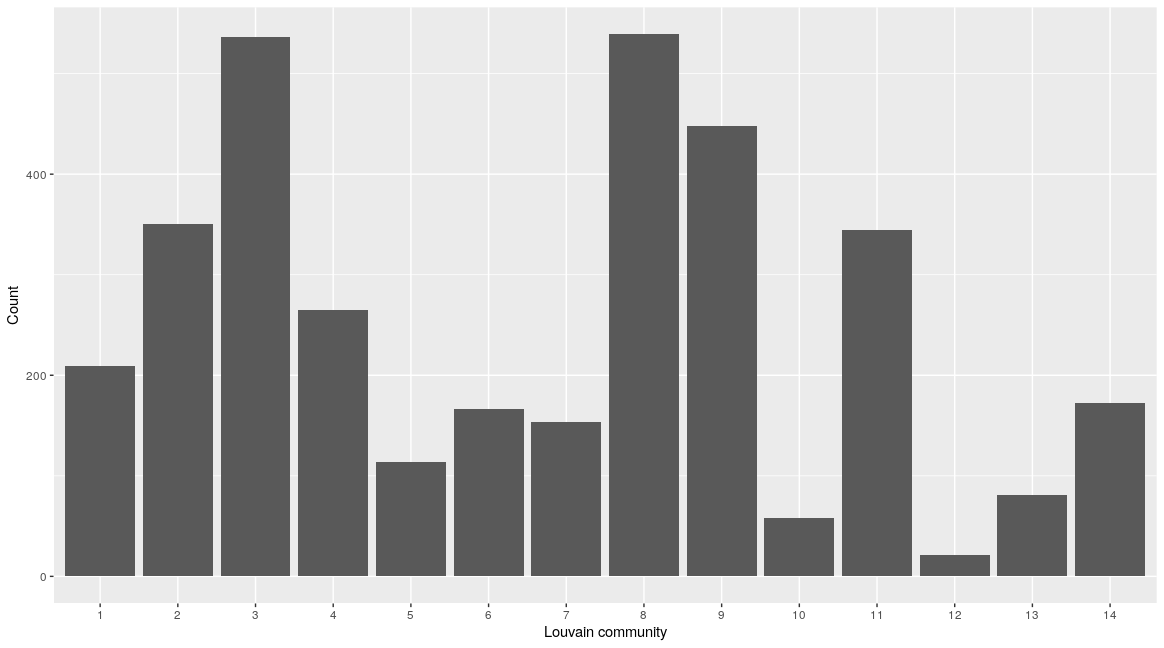
\includegraphics[width=\textwidth]{images/Rplot_Louvain_community_sizes.png}
    \caption{Barplot of the size of communities from the PSP discovered using the Louvain clustering method implemented in igraph}
    \label{fig:barplot_size_commmunities_using_louvain}
\end{figure}

Group 7 shows enrichment in the intelligence discovery (p=0.0012) and replication cohorts (p=0.0026). Group 7 is composed of 154 genes but the number shown in the tables of results may be less than this if a gene was not assigned any SNPs using MAGMA. Using a discovery and replication cohort alpha is 0.0125, but the enrichment is greater than considering all of the groups alpha 0.00357 (0.05/14). See table~\ref{tab:Louvain clustering intelligence}

Group 7 is enriched in the discovery cohort for education but not the replication cohort (p=0.0146 and replication p=0.4750). See table~\ref{tab:Louvain clustering education}.

Using the largest cohorts available for intelligence we confirm group 7 is enriched (Savage) p=0.0002. Two other groups survive multuple testing at alpha corrected for all groups see table~\ref{tab:Louvain clustering Savage intelligence phase 2 cohorts}. 

Using the largest cohorts available for education we find enrichment of group 7 (p=0.0017) and the group 8 found in Savage (p=0.0003) see table~\ref{tab:Louvain clustering EA3 Education cohorts}
% latex table generated in R 3.6.1 by xtable 1.8-4 package
% Sat Mar 28 15:46:38 2020

Group 7 is enriched for Molecular function glutamate receptor activity GO:0008066 	glutamate receptor activity 		 	Bonferroni (against genome) $3.478 \times 10^{-32}$ 	Number in group 26  In annotation	84. 
Group 8 is large. The second most enriched Biological process is GO:0048666 	neuron development 		Bonferroni	$1.180 \times 10^{-52}$ 	Number in group 150 	Number in annotation 1298.

Code on mac \url{source('~/RProjects/utils/src/generic_compile_gsa_lourvain_new.R')}
\todo{Overlap of group 7 with group 5}
\begin{table}[ht]
\centering
\begin{tabular}{rlrrrrrr}
  \hline
 & SET & NGENES & BETA & BETA\_STD & SE & Intelligence Discovery & Intelligence Replication \\ 
  \hline
2 & 2::: & 334 & 0.09 & 0.01 & 0.05 & 0.0407 & 0.1916 \\ 
  3 & 3::: & 510 & 0.10 & 0.02 & 0.04 & 0.0075 & 0.1006 \\ 
  7 & 7::: & 144 & 0.26 & 0.02 & 0.08 & 0.0012 & 0.0026 \\ 
  12 & 12::: & 21 & 0.63 & 0.02 & 0.21 & 0.0014 & 0.1628 \\ 
   \hline
\end{tabular}
\caption{Louvain clustering PSP Intelligence cohorts}
\label{tab:Louvain clustering intelligence}
\end{table}

% ed

% latex table generated in R 3.6.1 by xtable 1.8-4 package
% Sat Mar 28 15:49:04 2020
\begin{table}[ht]
\centering
\begin{tabular}{rlrrrrrr}
  \hline
 & SET & NGENES & BETA & BETA\_STD & SE & P & P\_EA2 \\ 
  \hline
2 & 2::: & 334 & 0.13 & 0.02 & 0.05 & 0.0071 & 0.0568 \\ 
  5 & 5::: & 112 & 0.23 & 0.02 & 0.09 & 0.0063 & 0.3478 \\ 
  7 & 7::: & 144 & 0.19 & 0.02 & 0.09 & 0.0146 & 0.4750 \\ 
   \hline
\end{tabular}
\caption{Louvain clustering PSP Education cohorts}
\label{tab:Louvain clustering education}
\end{table}

% latex table generated in R 3.6.1 by xtable 1.8-4 package
% Sat Mar 28 15:51:04 2020 Sav2
\begin{table}[ht]
\centering
\begin{tabular}{rlrrrrr}
  \hline
 & SET & NGENES & BETA & BETA\_STD & SE & P \\ 
  \hline
2 & 2::: & 345 & 0.11 & 0.02 & 0.0550 & 0.0208 \\ 
  3 & 3::: & 527 & 0.11 & 0.02 & 0.0431 & 0.0055 \\ 
  7 & 7::: & 153 & 0.32 & 0.03 & 0.0899 & 0.0002 \\ 
  8 & 8::: & 537 & 0.14 & 0.02 & 0.0475 & 0.0018 \\ 
   \hline
\end{tabular}
\caption{Louvain clustering PSP Savage Intelligence phase2 cohorts}
\label{tab:Louvain clustering Savage intelligence phase 2 cohorts}
\end{table}


% latex table generated in R 3.6.1 by xtable 1.8-4 package
% Sat Mar 28 15:52:19 2020
\begin{table}[ht]
\centering
\begin{tabular}{rlrrrrr}
  \hline
 & SET & NGENES & BETA & BETA\_STD & SE & P \\ 
  \hline
1 & 1::: & 196 & 0.11 & 0.01 & 0.0897 & 0.1185 \\ 
  2 & 2::: & 334 & 0.06 & 0.01 & 0.0660 & 0.2021 \\ 
  3 & 3::: & 510 & 0.08 & 0.01 & 0.0521 & 0.0740 \\ 
  4 & 4::: & 245 & 0.10 & 0.01 & 0.0792 & 0.0943 \\ 
  5 & 5::: & 111 & 0.09 & 0.01 & 0.1110 & 0.2132 \\ 
  6 & 6::: & 159 & 0.01 & 0.00 & 0.0958 & 0.4421 \\ 
  7 & 7::: & 144 & 0.32 & 0.03 & 0.1080 & 0.0017 \\ 
  8 & 8::: & 519 & 0.19 & 0.03 & 0.0558 & 0.0003 \\ 
  9 & 9::: & 425 & 0.04 & 0.01 & 0.0640 & 0.2426 \\ 
  10 & 10::: & 57 & 0.03 & 0.00 & 0.1570 & 0.4303 \\ 
  11 & 11::: & 331 & 0.08 & 0.01 & 0.0679 & 0.1087 \\ 
  12 & 12::: & 21 & -0.11 & -0.00 & 0.2620 & 0.6587 \\ 
  13 & 13::: & 80 & -0.12 & -0.01 & 0.1330 & 0.8143 \\ 
  14 & 14::: & 166 & 0.09 & 0.01 & 0.0989 & 0.1692 \\ 
   \hline
\end{tabular}
\caption{Louvain clustering PSP EA3 Education cohorts}
\label{tab:Louvain clustering EA3 Education cohorts}
\end{table}

\begin{table}[]
    \centering
    \begin{tabular}{cc}
    \toprule
        Method & Q \\
        \midrule
        Spectral & 0.30\\
        Infomap & 0.275\\
        Louvain & 0.339\\
        Lec & 0.247\\
        walk trap & 0.256\\
        \bottomrule
    \end{tabular}
    \caption{Modularity using different partion methods}
    \label{tab:modularity}
\end{table}

\section{Infomap}

Infomap works using information theory about random walks. It is implemented in igraph for R. 

There are no free parameters that need to be supplied

\subsection{Results}

Infomap discovers 171 communities. Group size  Min. 1st 2.00 Qu.5.00   Median 8.00     Mean 20.22 3rd Qu. 13.00   Max. 1228.00

One group is responsible for 35.5\% of the PSP. 916 nodes belonged to 134 groups less than size 15. 36 groups had communities greater than or equal to 15 and smaller than the largest group (1313 genes). The second largest group has 130 members.  

The modularity of the partition is 0.275.


For intelligence cohort see table~\ref{tab:Infomap Intelligence infomap significant in both groups}

For education cohort see table~\ref{tab:infomap education}. For the large new cohorts in education (EA3) see table~\ref{tab:infomap EA3} and intelligence (Savage) see table~\ref{tab:Infomap savage}.

Group 11 consists of NMDA receptors and DLG genes. The disease most associated with it is ASD. Group 1 is large limiting enrichment analysis but RNA binding GO:0003723 in 406 genes P Bonferroni against all genome $2.728 \times 10^{-112}$ \subsection{Overlap with other partitions}

Group 5 Spectral was distributed quite widely but there were 31 in group 16, 10 in 21 and 19 in 24 using infomap. Group 24 is enriched in the savage study and contains GRIP1, GRIA 1-4, GRIK 1,2,3,5, 3 metabotropic, PICK1, GRIP AP and CACNG2. This seems to be a cohesive group across different clusterings (see below) code \url{source('~/RProjects/graph2community/R/overlap_info.R')}

\todo{take 1 neighbourhood of these genes}

For the overlap between group 5 and louvain group 7 22 were in group 7 and 57 in Louvain 14.

The 22 gene overlap between group 5 and louvain group 7 were ampa, kainate and 3 metabotropic glutamate along with PICK1 and GRIP AP1 and a few others. GSA 13 glutamate receptor activity GO:0008066 

This supports the Newman idea that different partitions are made up of similar components. 

\todo{can add that infomap and Louvain along with spectral are the ones most recommended by Newman and that group has expertise with spectral also to add and look at overlap for block stochastic.}

% latex table generated in R 3.6.1 by xtable 1.8-4 package
% Tue Mar 31 13:59:17 2020 int



\begin{table}[ht]
\centering
\begin{tabular}{rlrrrrrr}
  \hline
 & SET & NGENES & BETA & BETA\_STD & SE & P & P\_C \\ 
  \hline
1 & 1::: & 1176 & 0.1 & 0.02 & 0.03 & 0.0061 & 0.0479 \\ 
  11 & 11::: & 47 & 0.4 & 0.02 & 0.15 & 0.0018 & 0.0080 \\ 
   \hline
\end{tabular}
\caption{Intelligence infomap significant in both groups}
\label{tab:Infomap Intelligence infomap significant in both groups}
\end{table}

% latex table generated in R 3.6.1 by xtable 1.8-4 package
% Tue Mar 31 14:05:51 2020
\begin{table}[ht]
\centering
\begin{tabular}{rlrrrrr}
  \hline
 & SET & NGENES & BETA & BETA\_STD & SE & P \\ 
  \hline
1 & 1::: & 1173 & 0.06 & 0.02 & 0.0364 & 0.0415 \\ 
  8 & 8::: & 62 & 0.39 & 0.02 & 0.1650 & 0.0096 \\ 
  11 & 11::: & 47 & 0.62 & 0.03 & 0.1990 & 0.0010 \\ 
  17 & 17::: & 22 & 0.57 & 0.02 & 0.2730 & 0.0191 \\ 
  23 & 23::: & 20 & 0.60 & 0.02 & 0.2880 & 0.0188 \\ 
  30 & 30::: & 15 & 0.54 & 0.02 & 0.2890 & 0.0313 \\ 
  31 & 31::: & 13 & 1.04 & 0.03 & 0.3900 & 0.0037 \\ 
  67 & 67::: &  7 & 0.64 & 0.01 & 0.3700 & 0.0422 \\ 
  68 & 68::: &  9 & 0.73 & 0.02 & 0.4060 & 0.0354 \\ 
  76 & 76::: &  8 & 1.37 & 0.03 & 0.5050 & 0.0033 \\ 
  98 & 98::: &  6 & 1.29 & 0.02 & 0.5320 & 0.0077 \\ 
  99 & 99::: &  7 & 0.80 & 0.02 & 0.4250 & 0.0299 \\ 
  111 & 111::: &  6 & 2.22 & 0.04 & 0.5960 & 0.0001 \\ 
  135 & 135::: &  4 & 2.26 & 0.03 & 0.7930 & 0.0022 \\ 
  139 & 139::: &  4 & 1.71 & 0.03 & 0.7020 & 0.0076 \\ 
  158 & 158::: &  2 & 2.20 & 0.02 & 0.9880 & 0.0129 \\ 
  161 & 161::: &  2 & 1.79 & 0.02 & 1.0500 & 0.0451 \\ 
  167 & 167::: &  2 & 1.54 & 0.02 & 0.7630 & 0.0220 \\ 
  170 & 170::: &  2 & 2.56 & 0.03 & 0.9150 & 0.0026 \\ 
   \hline
\end{tabular}
\caption{Significant EA3 infomap}
\label{tab:infomap EA3}
\end{table}

% latex table generated in R 3.6.1 by xtable 1.8-4 package
% Tue Mar 31 14:07:01 2020
\begin{table}[ht]
\centering
\begin{tabular}{rlrrrrrr}
  \hline
 & SET & NGENES & BETA & BETA\_STD & SE & P & P\_EA2 \\ 
  \hline
99 & 99::: &  7 & 0.7 & 0.01 & 0.36 & 0.0211 & 0.0428 \\ 
  106 & 106::: &  6 & 0.8 & 0.01 & 0.47 & 0.0452 & 0.0021 \\ 
  135 & 135::: &  4 & 1.6 & 0.02 & 0.61 & 0.0038 & 0.0070 \\ 
   \hline
\end{tabular}
\caption{Education infomap}
\label{tab:infomap education}
\end{table}

% latex table generated in R 3.6.1 by xtable 1.8-4 package
% Tue Mar 31 14:07:31 2020
\begin{table}[ht]
\centering
\begin{tabular}{rlrrrrr}
  \hline
 & SET & NGENES & BETA & BETA\_STD & SE & P \\ 
  \hline
1 & 1::: & 1213 & 0.08 & 0.02 & 0.0304 & 0.0061 \\ 
  8 & 8::: & 65 & 0.27 & 0.02 & 0.1370 & 0.0231 \\ 
  12 & 12::: & 41 & 0.29 & 0.01 & 0.1460 & 0.0249 \\ 
  18 & 18::: & 31 & 0.45 & 0.02 & 0.1930 & 0.0093 \\ 
  19 & 19::: & 27 & 0.53 & 0.02 & 0.2330 & 0.0120 \\ 
  24 & 24::: & 22 & 0.68 & 0.02 & 0.2370 & 0.0019 \\ 
  42 & 42::: & 13 & 0.70 & 0.02 & 0.2770 & 0.0057 \\ 
  49 & 49::: & 11 & 0.61 & 0.01 & 0.3240 & 0.0307 \\ 
  50 & 50::: & 12 & 1.11 & 0.03 & 0.3310 & 0.0004 \\ 
  62 & 62::: & 12 & 0.58 & 0.01 & 0.2770 & 0.0176 \\ 
  74 & 74::: &  9 & 0.94 & 0.02 & 0.3740 & 0.0061 \\ 
  76 & 76::: &  8 & 1.20 & 0.02 & 0.4310 & 0.0027 \\ 
  77 & 77::: &  8 & 0.95 & 0.02 & 0.4550 & 0.0187 \\ 
  96 & 96::: &  7 & 1.54 & 0.03 & 0.4380 & 0.0002 \\ 
  101 & 101::: &  8 & 0.80 & 0.02 & 0.4210 & 0.0294 \\ 
  111 & 111::: &  6 & 1.09 & 0.02 & 0.5420 & 0.0223 \\ 
  120 & 120::: &  6 & 0.68 & 0.01 & 0.4070 & 0.0476 \\ 
  135 & 135::: &  4 & 2.11 & 0.03 & 0.6740 & 0.0009 \\ 
  158 & 158::: &  2 & 2.03 & 0.02 & 0.8370 & 0.0077 \\ 
  170 & 170::: &  2 & 3.06 & 0.03 & 0.9540 & 0.0007 \\ 
   \hline
\end{tabular}
\caption{Savage infomap}
\label{tab:Infomap savage}
\end{table}

\section{Walk trap}

Implemented in igraph. 562 communities , 405 have single member  Min.1 1st Qu.  1 Median1    Mean 6.151 3rd Qu. 2   Max. 760 
 
  
\section{Spinglass}

There are a number of tunable parameters for the implementation of the spinglass algorithm in igraph for R specifically
args for spinglass
\begin{itemize}
    \item{weights not applicable - edge weights}
    \item vertex - community for specific vertex ignore
    \item spins default 25 - upper limit for number of communities
    \item parupdate false not required
    \item start.temp default 1
    \item stop.temp 0.1
    \item cool.fact for simulated annealing
    \item update simple or random or config we may need config
    \item gamma = balance between present and non present edges in a community present and non present edges default 1.0 makes existing and non existing links equally important, smaller make existing links, greater missing links more important
\end{itemize}









\todo{Check enrichment}


\subsection{Theory behind spinglass}
\todo{remember local clustering}
\todo{remember reasons for looking for communities around or less than 100 Leskovec paper on peak conductance}

\subsection{Implementation}
Spin glass clustering was carried out using the igraph package in R using a script to automatically generate values for gamma and spins and to conver the communities object into a graph markup language(GML) file. 5 gamma values were used gamma = $0.1,0.5,1,2,5$ and 9 spin values spins = $2,10,20,30,40,50,60,80,100$ 
Running 45 grid search the clustering with spinglass takes about 56.6 seconds which accumulates if one has a large number of clusters to make therefore Grid search generation run on staff.compute R 3.5 DICE.
Gamma of 0.1 and 0.5 only returned valid spins of 2 and 2,10 respectively. 
\subsection{Study design}
Given the number of tunable parameters in the spinglass model it is difficult to make a study design similar to that we used with the spectral clustering as the number of communities will lead to a prohibitively small alpha level. The possibility of finding individual datasets for each set of communities at each parameter setting is not practicable as even varying only gamma and spins we have the cartesian product of the number of parameter settings numbers of groups of sets.

The number of spins controls the maximum number of groups found in the clustering. The value of gamma controls the importance of there being edges present within the commmunity modules.

We would however prefer not to abandon spin glass entirely. McLean (personal commmunication) found it gave good community enrichment at certain values (higher values) of gamma. However we are also aware both from theory and our earlier experiment that pure modules in the ontology sense may not be what we want. We may want a dominant ontology group and their neighbouring proteins that form a module as this may map more reliably onto population data. Also although it is attractive the ontology group is in no sense a ground truth it is still 'Menschenwerk' (Kronecker).

One option is to adopt a strategy from machine learning. We will define the discovery intelligence and education as the training set and find the groups of sets that have a set with an arbitrarily low p value and of a satisfactory size. We will then combine these into a group of sets and test these on the replication cohorts. The design is not so robust as the previous one but at least allows us to see what insights we might gain from the spin glass clustering. We are not randomly sampling from the synaptic proteome there is still the constraint that we require that the sets form modules (in terms of their edge in-out distribution) and that the modules are connected subgraphs of the network. The arbitrary element (or the most arbitrary element) of this design is the choice of alpha. We want to chose alpha such that the number of sets to test in the replication does not lead to excessive type II error. The lower we choose alpha for the first set the more likely the p value of the second set is to be low. We can also try using the nominal alpha level of 0.5 and see what we get. 

\subsubsection{Spinglass results}
We get significant enrichment for spin 2 gamma 5 for education and intelligence both sets. This is because we are splitting the PSD in two. The larger approx 2082 number of genes is the one that enriches.

For spins 10 gamma 5 we get 10 groups the 417 number group enriches strongly in discovery and replication but not for education and it is a big group.



\todo{Modularity}
\subsection{Modularity}

Although the modularity of a partition of random graph tends towards 0 we can calculate the modularity of a randomly wired graph with the pre-existing group allocations \footnote{\url{source('~/RProjects/centrality/R/bootstrap_ci_modularity.R')}}

We can also calculate the modularity for clustering a random graph. Louvain 1000 iterations.
  Min. 1st Qu.  Median    Mean 3rd Qu.    Max. 
 0.1468  0.1577  0.1602  0.1601  0.1627  0.1706 
 
 distribution of results near normal. 	Shapiro-Wilk normality test

data:  results
W = 0.99726, p-value = 0.0877

Mean centred = same 0.0877

The degree distribution is part of the results. 

The values are lower using random degree sequences but not all are valid here is an example we would have to do try except better in python \footnote{\url{source('~/RProjects/centrality/R/bootstrap_ci_modularity_louvain_cluster_resampling.R')}}

   Min. 1st Qu.  Median    Mean 3rd Qu.    Max. 
 0.1427  0.1504  0.1529  0.1527  0.1552  0.1626 
 
 Barabsi.game with n=3457 and gamma = 2.7
 \footnote{\url{source('~/RProjects/centrality/R/bootstrap_ci_modularity_louvain_cluster_barabasi.R')}}
 

\textcolor{red}{It is significantly enriched for glutamate receptor activity (37 of 84) and axon guidance and for ASD, schizophrenia and seizures \todo{overlap with group 5}. It also enriches significantly in EA3 group 5(Spinglass) $P=0.0010319$ but so does group 9 at p=$0.0014555$ src \url{source('~/RProjects/gridsearch_gamma/R/check_results/check_results.R')}
Enriches strongly in savage $0.0049343$ but less so in davies (approx 0.02 but group 4 very strongly in davies)}

\section{SBM}
See core periphery

 \section{Community detection thresholds}
There are limits to the detection of communities specifically in the difference between the probability of edges and the probability of in group edges.
 
 \section{Enrichment of the presynaptic proteome}
 
 Surprisingly all of the education phenotypes enrich for genes in the presynaptic proteome and this is not true of intelligence except weakly for UKBB Intelligence Discovery. The reasons for this are unclear. See figure \ref{Table:Enrichment of intelligence phenotypes presynaptic proteome} and \ref{Table:Enrichment of education phenotypes presynaptic proteome}
 
 % latex table generated in R 3.6.1 by xtable 1.8-4 package
% Thu Jan 16 16:01:27 2020
\begin{table}[ht]
\centering
\begin{tabular}{rlrrrrr}
  \hline
 & SET & NGENES & BETA & BETA\_STD & SE & P \\ 
  \hline 

1 & Education Replication\_presynaptic\_all & 1449 & 0.06 & 0.02 & 0.02 & 0.00 \\ 
  2 & Education Discovery\_presynaptic\_all & 1461 & 0.07 & 0.02 & 0.03 & 0.00 \\ 
  3 & EA3\_presynaptic\_all & 1460 & 0.10 & 0.03 & 0.03 & 0.00 \\ 
   \hline
\end{tabular}
\caption{Enrichment of education phenotypes presynaptic proteome} 
\label{Table:Enrichment of intelligence phenotypes presynaptic proteome}
% latex table generated in R 3.6.1 by xtable 1.8-4 package
% Thu Jan 16 16:01:27 2020
\end{table}

\begin{table}
\centering
\begin{tabular}{rlrrrrr}
  \hline
 & SET & NGENES & BETA & BETA\_STD & SE & P \\ 
  \hline
1 & Education Replication\_presynaptic\_all & 1449 & 0.06 & 0.02 & 0.02 & 0.0048 \\ 
  2 & Education Discovery\_presynaptic\_all & 1461 & 0.07 & 0.02 & 0.03 & 0.0032 \\ 
  3 & EA3\_presynaptic\_all & 1460 & 0.10 & 0.03 & 0.03 & 0.0020 \\ 
   \hline
\end{tabular}
\caption{Enrichment of education phenotypes presynaptic proteome} 
\label{Table:Enrichment of education phenotypes presynaptic proteome}
\end{table}


% latex table generated in R 3.6.1 by xtable 1.8-4 package
% Thu Jan 16 16:01:27 2020
\begin{table}[ht]
\centering
\begin{tabular}{rlrrrrr}
  \hline
 & SET & NGENES & BETA & BETA\_STD & SE & P \\ 
  \hline
1 & Intelligence Discovery\_presynaptic\_all & 1461 & 0.05 & 0.01 & 0.03 & 0.04 \\ 
  2 & Intelligence Replication\_presynaptic\_all & 1466 & 0.02 & 0.00 & 0.02 & 0.23 \\ 
  3 & Savage\_presynaptic\_all & 1498 & 0.04 & 0.01 & 0.03 & 0.10 \\ 
  4 & Davies\_presynaptic\_all & 1460 & 0.05 & 0.01 & 0.03 & 0.04 \\ 
   \hline
\end{tabular}
\caption{Enrichment of intelligence phenotypes presynaptic proteome} 
\label{Table:Enrichment of intelligence phenotypes presynaptic proteome}
\end{table}

% latex table generated in R 3.6.1 by xtable 1.8-4 package
% Thu Jan 16 16:01:27 2020
\begin{table}[ht]
\centering
\begin{tabular}{rlrrrrr}
  \hline
 & SET & NGENES & BETA & BETA\_STD & SE & P \\ 
  \hline 

1 & Intelligence Discovery\_presynaptic\_all & 1461 & 0.05 & 0.01 & 0.03 & 0.04 \\ 
  2 & Intelligence Replication\_presynaptic\_all & 1466 & 0.02 & 0.00 & 0.02 & 0.23 \\ 
  3 & Savage\_presynaptic\_all & 1498 & 0.04 & 0.01 & 0.03 & 0.10 \\ 
  4 & Davies\_presynaptic\_all & 1460 & 0.05 & 0.01 & 0.03 & 0.04 \\ 
   \hline
\end{tabular}
\caption{Enrichment of intelligence phenotypes presynaptic proteome \url{'~/RProjects/paper_xls_output/R/make_pLI_correlation}...., line 507} 
\label{Table:Enrichment of intelligence phenotypes presynaptic proteome}
\end{table}

Those of low betweeness are a slightly smaller group but enrich more in ea2 and ukbbed. Todo correlation of graph degree etc and study in presynaptic. \url{source('~/RProjects/graph_distances/R/collate_presynaptic_edubet.R')}
 

The most enriched genes in toppgene are labelled as post synaptic including BSN, SHANK3 and CAMKV. There is overlap between presynaptic and PSP (\todo{how much overlap}) A large number of the highest scoring presynaptic genes are listed as post synaptic in toppgene. \todo{MAGMA GSA for toppgene presynaptic genes}

\todo{what are setgenesout for all post synaptic or murine}